\chapter{Methodology}\label{chap:Methodology}

\begin{center} 
  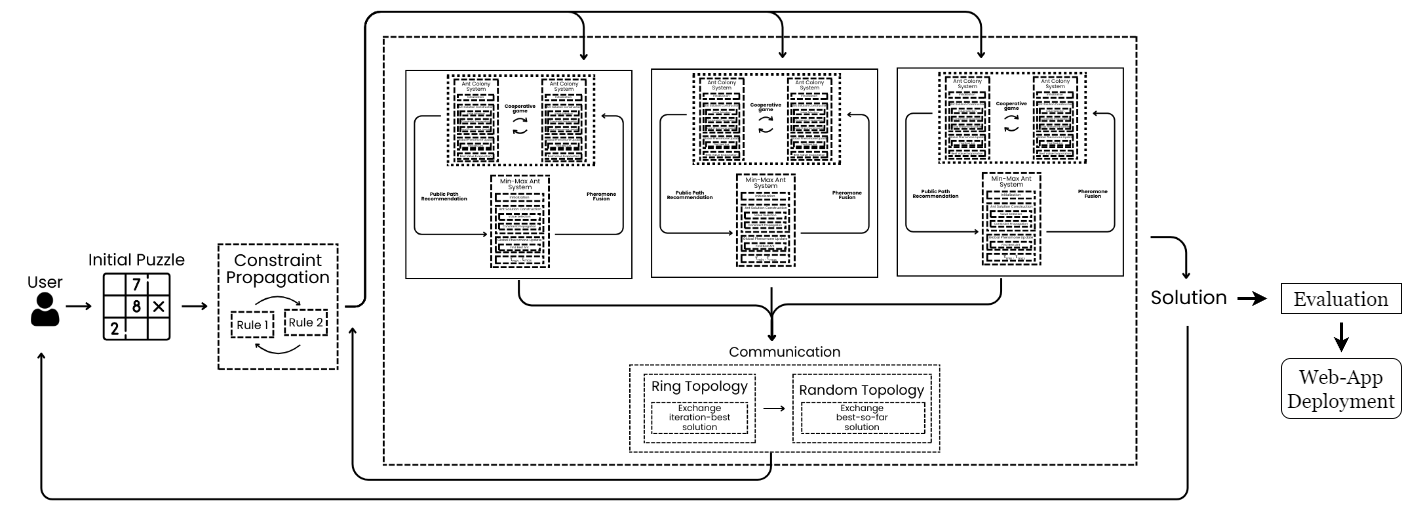
\includegraphics[width=\linewidth]{../figures/General Overview.png} 
  \captionof{figure}{General methodology overview} 
  \label{general} 
\end{center}

Figure~\ref{general} shows the general overview of the methodology from data gathering to model deployment. Inputting the sudoku puzzles retrieved from publicly available dataset with different sizes and number of clues into the constraint propagation defines the initial step of the process. Constraint propagation removes infeasible solutions thus reducing the search space through naked single elimination. After that, the proposed model, collaborative multithreaded multi-colony ant optimization, receives the refined puzzle. The collaborative mechanism between threads is periodically activated to enhance the search process for a valid solution. The execution is terminated when there are any threads who successfully generate a valid sudoku solution.  The proposed model is then evaluated based on performance metrics namely solution success rate, average completion time, standard deviation, and average number of cycles. 

\section{Dataset}
The study used a large pool of publicly available sudoku instances with sizes 9 x 9 and 16 x 16. The proposed solver is then used to solve these puzzles and selected 100 most difficult instances for the final benchmark instances. The selection was based on the computational effort and solving time of the solver. For large 25 x 25 grids, sudoku instances of this size were obtained from the work of Lloyd and Amos~\cite{lloyd2020}. The final benchmark dataset is composed of 300 sudoku instances with 100 instances for each puzzle size. 
            
All these sudoku puzzles are stored in a text file that includes the position of the clues. The  ratio between the number of clues and the puzzle size defined the complexity of the puzzle. 

        \begin{figure}[H]
            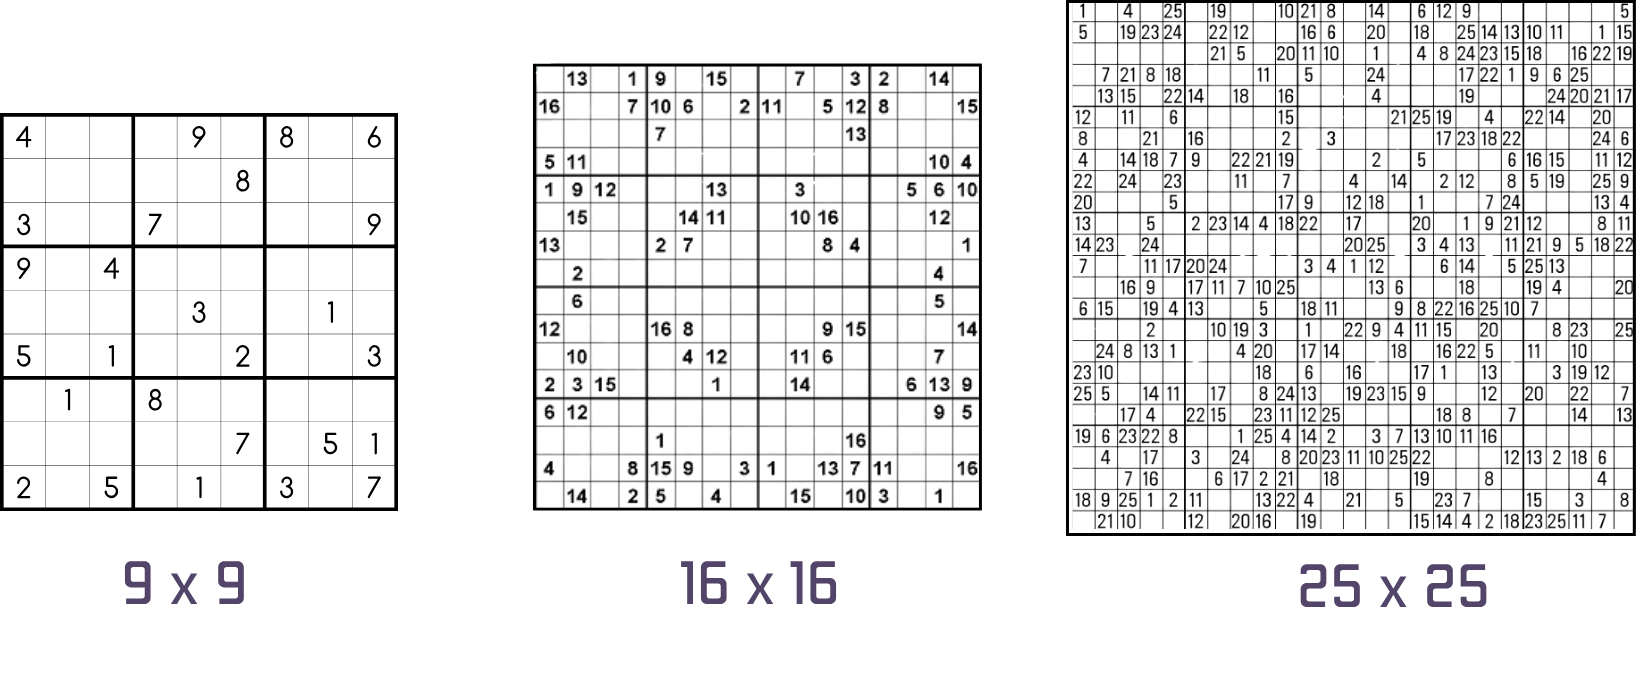
\includegraphics[width=\linewidth]{../figures/Dataset.png}
            \centering
            \caption{Shows different sudoku puzzle sizes.}\label{dataset}
        \end{figure}

\subsubsection*{File Format}
The sudoku instances are stored in text file with a specific layout. The first integer found in the first line of the input text file refers to the size of the subgrid from the puzzle. It is the order of the puzzle ($N = \text{order}^2$)
        \begin{itemize}
            \item ``3'' - refers to a $9 \times 9$ Sudoku puzzle.
            \item ``4'' - refers to a $16 \times 16$ Sudoku puzzle.
            \item ``5'' - refers to a $25 \times 25$ Sudoku puzzle.
        \end{itemize}


%However, the first integer found in the first line of the sudoku puzzle instances with sizes $6 \times 6$ and $12 \times 12$ refers to the size of the puzzle itself and not the size of the subgrid anymore. 
%        \begin{itemize}
%            \item ``6'' - refers to a $6 \times 6$ Sudoku puzzle.
%            \item ``12'' - refers to a $12 \times 12$ Sudoku puzzle.
%        \end{itemize}

The second integer found in the second line of the input text file is just a placeholder. It is not utilized by the solver. Lastly, the integers found starting from the third line refers to the puzzle itself. It is a mixture of positive numbers from 0 to $N$ and $-1$ as shown in Figure~\ref{puzzleInit}. Empty cells are represented by $-1$.  

        \begin{figure}[H]
            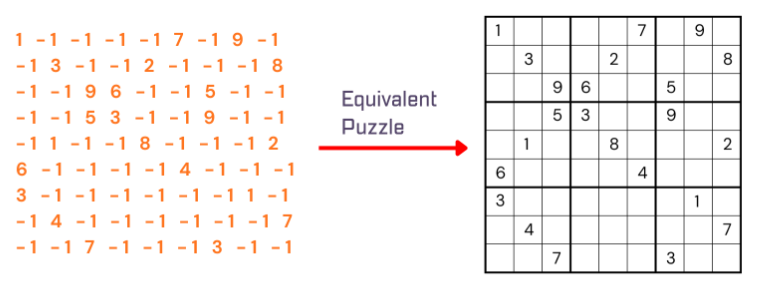
\includegraphics[width=\linewidth]{../figures/inputFile.png}
            \centering
            \caption{Example of a Raw Input File to its equivalent Puzzle}\label{puzzleInit}
        \end{figure}


\section{SudoSLVRR: Design and Structure}

\subsection{Constraint Propagation}
The constraint propagation (CP) is the one that acts like a preprocessing step of the proposed  multithreaded multi-colony ant optimization model with ring and random communication topologies. It narrows down the search space as it removes infeasible cell-digit assignments before the optimization begins. In the context of Sudoku, rules are established and should be followed. Each cell must contain only one digit while satisfying these three simultaneous constraints:
        \begin{enumerate}
            \item \textbf{Row Constraint} - Each number from 1 to {$n$} must occur exactly once in every row. 
            \item \textbf{Column Constraint} - Each number from 1 to {$n$} must occur exactly once in every column.
            \item\textbf{Subgrid Constraint} - Each number from 1 to {$n$} must occur exactly once within each subgrid or region.
        \end{enumerate}

It is the constraint propagation who makes sure that these three constraints are satisfied. Initially, CP assumes all the numbers from 1 to n are possible for every empty cell as shown in Figure~\ref{valueSet}. As we all know, the sudoku puzzle has clues before it was even fed to CP. For every cell in the puzzle, it contains candidate values which is a set of values that is possible to be assigned in the cell.

        \begin{figure}[H]
            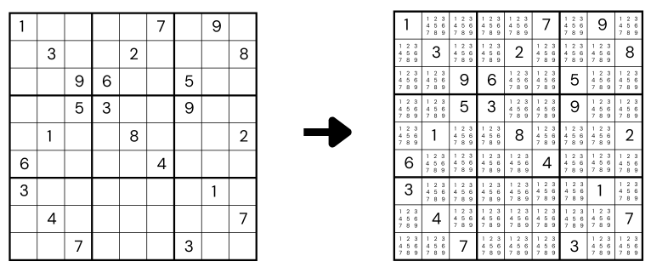
\includegraphics[width=\linewidth]{../figures/ValueSet.png}
            \centering
            \caption{ValueSet Representation for AI Escargot}\label{valueSet}
        \end{figure}\

In removing invalid assignments, CP implements two rules. In rule 1, CP checks every cell and its peers (other cells that reside in the same row, column, and subgrid). CP removes the values from the candidate values that are already fixed in the cell’s peers as shown in Figures~\ref{fig:cp_step_1a} and~\ref{fig:cp_step_1b}. It is done by having two sets where one contains all the candidate values for the checked cell and the other contains the union of all the values that are already fixed in that cell’s peers. Then it uses set difference to remove invalid assignments for the checked cell. 

\begin{center}
    \begin{minipage}{\linewidth}
        \centering
        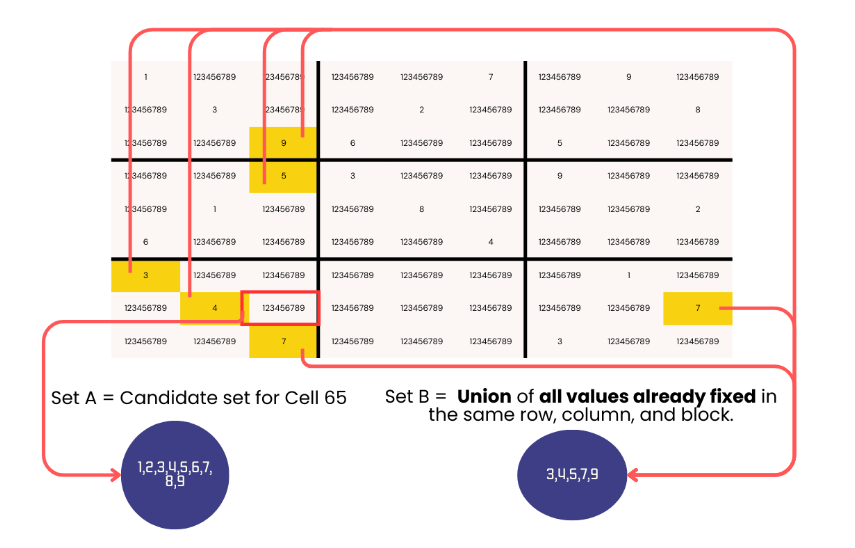
\includegraphics[width=0.8\linewidth]{../figures/CP Rule 1 a.png} 
        \captionof{figure}{Before applying CP Rule 1} 
        \label{fig:cp_step_1a} 
        
        \vspace{1.0cm} % Slightly smaller gap
        
        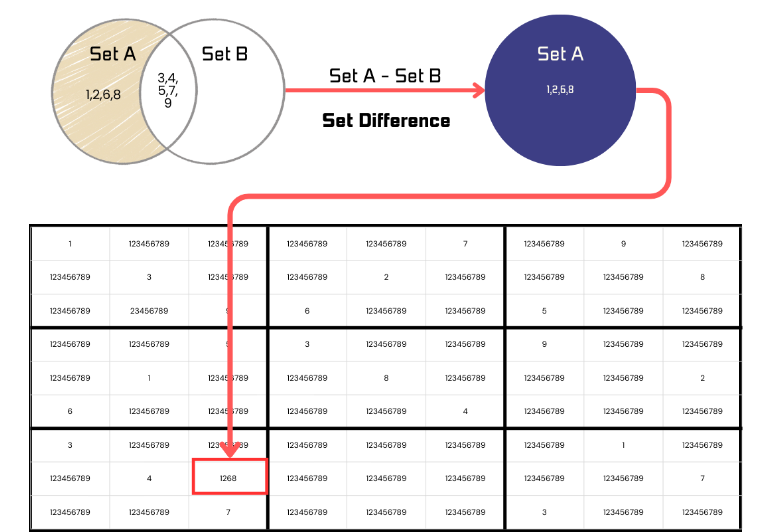
\includegraphics[width=0.8\linewidth]{../figures/CP Rule 1 b.png} 
        \captionof{figure}{After applying CP Rule 1} 
        \label{fig:cp_step_1b} 
    \end{minipage}
\end{center}

The second rule being implemented by the CP is often called as \textbf{hidden single elimination}.

\begin{center}
    \begin{minipage}{\linewidth}
        \centering
        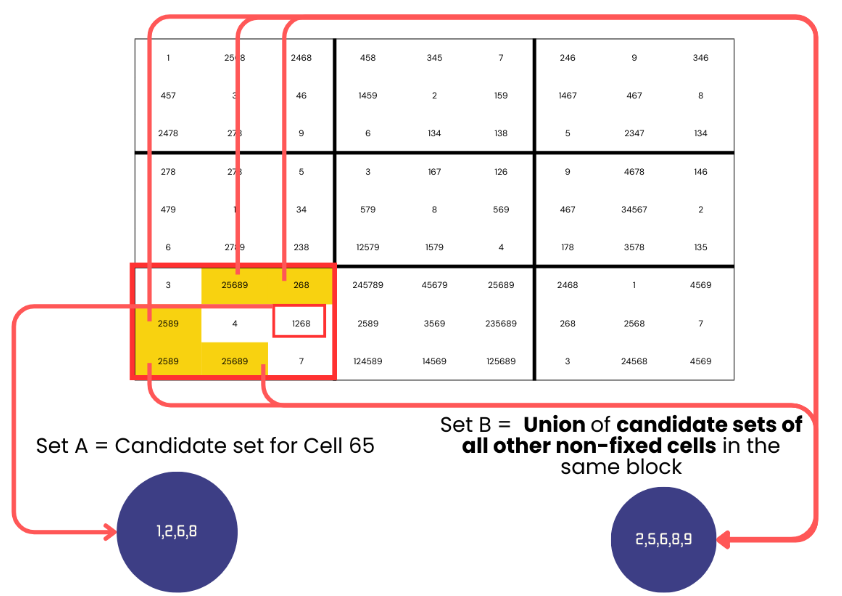
\includegraphics[width=0.8\linewidth]{../figures/CP Rule 2 a.png} 
        \captionof{figure}{Before applying CP Rule 2} 
        \label{fig:cp_step_2a} 
        
        \vspace{1.0cm} % Slightly smaller gap
        
        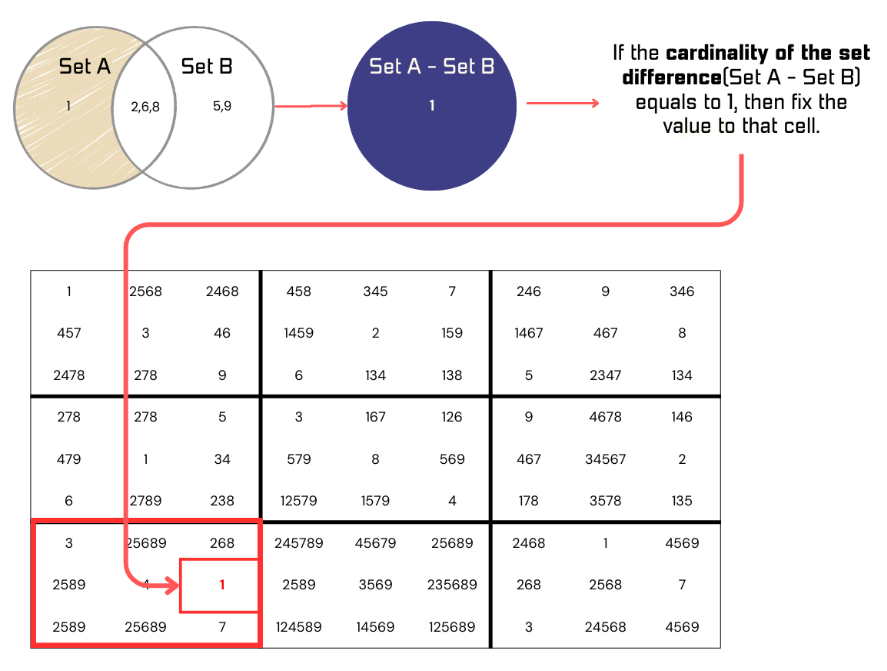
\includegraphics[width=0.8\linewidth]{../figures/CP Rule 2 b.png} 
        \captionof{figure}{After applying CP Rule 2} 
        \label{fig:cp_step_2b} 
    \end{minipage}
\end{center}

When there is a candidate value that can go only to one cell after the CP applied the row, column, and subgrid constraints, then that cell is known to have a hidden single as shown in Figure~\ref{fig:cp_step_2b}. This is done by having two sets where one contains all the candidate values for the checked cells while the other one contains the union of all the candidate values found from the checked cell’s peers. If the cardinality of the set difference equals to 1, then CP will immediately fix the hidden single value to that cell even though the checked cell has other candidate values. 

This process of elimination of values is repeated until no further logical deductions can be made. The output from the CP is shown in Figure~\ref{CP_result}. The base solver of this study, CP-DCM-ACO, which will be discussed in the next section, only focuses on feasible solutions thereby avoiding any infeasible solutions. Because of this, optimization will have to focus on finding valid solutions thus reducing computational time and the number of cycles it needs. 

\begin{center} 
  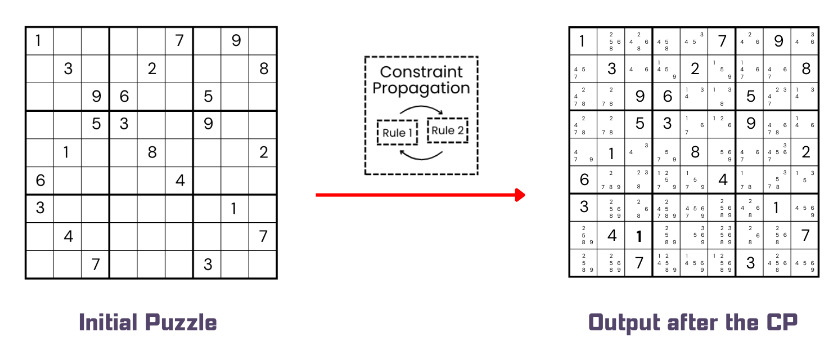
\includegraphics[width=\linewidth]{../figures/CP Result.png} 
  \captionof{figure}{Image from left is the AI Escargot instance and the right shows the result after CP} 
  \label{CP_result} 
\end{center}

\subsection{Initialization}
The proposed framework starts with the initialization phase where necessary variables should be set before any construction of solution begins. These variables are the necessary components as it affects the overall performance of the solver. 

    \begin{enumerate}
        \item \textbf{Number of Threads} - This includes the threads setup and its number. Threads are the one holding the main solver in this framework.
        \item \textbf{stopFlag} - This shared boolean flag is very important in terminating all the independent threads from working. When a solution is found from any of the threads or time limit is already exhausted, this flag will be set to true signaling all threads to stop. 
        \item\textbf{Communication Interval} - This is a parameter for multithreading that dictates when the threads should communicate. Adapted from~\cite{yang2015}, the interval is a non-fixed pattern as there is a long interval and a short interval. 
    \end{enumerate}

  As mentioned earlier, threads contain the main solver for the Sudoku Problem. As soon as the initialization of threads are done, the initialization of the necessary components of the main solver is executed.
    
    \begin{enumerate}
        \item \textbf{Colonies Initialization} - ACS and MMAS colonies are used from~\cite{mo2022}. ACS is known for its exploitation mechanism while MMAS has its exploratory characteristic. They differ on how they select a value. Also, MMAS has pheromone value boundaries while ACS has a best value evaporation. Included in this initialization are the number of ants, $q_0$, evaporation rate, best value evaporation, and the thresholds that dictate when does the communication between colonies happens. 
        \item \textbf{Pheromone Matrices} - Ants are pheromone-driven agents. They base their choices from the pheromone levels. The initial value of the pheromones (See Figure~\ref{PherInit}) is given by: 
        
        \begin{equation}
            \tau_{0} = \frac{1}{numCells}
        \end{equation}

        \begin{figure}[H]
            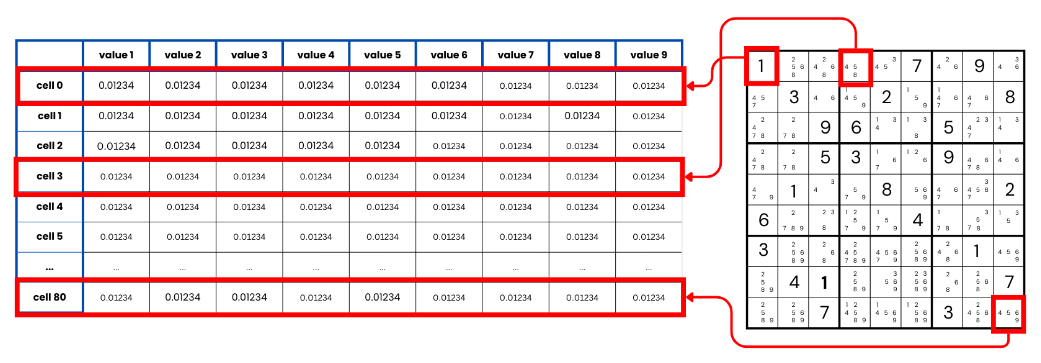
\includegraphics[width=0.9\textwidth]{../figures/PherMatrixInit.png}
            \centering
            \caption{Initial Pheromone Matrix for $9\times9$ Sudoku Puzzle}\label{PherInit}
        \end{figure}
        
    \end{enumerate}

\subsection{CP-DCM-ACO}
  In this study, the proposed framework implements multiple threads; each thread runs an independent instance of CP-DCM-ACO. This is the main solver of this framework and it integrates the constraint propagation and the dynamic collaborative multi-colony ant optimization. As mentioned earlier, constraint propagation is adapted from Lloyd and Amos~\cite{lloyd2020}. The dynamic collaborative multi-colony ant optimization (DCM-ACO) is adapted from the work of  Mo et al.~\cite{mo2022} where there is a cooperation between heterogeneous colonies of ant. 

  The popular problem where the ant colony system is used to solve is called Travelling Salesman Problem (TSP). Ants in this problem travel between cities and keep the path information. However in the context of Sudoku, the ``path'' that the ants keep is the cells visited and the value assigned to that cell by them. But before the ants begin their tour, the CP removes first any invalid assignments of values to cells. Because of this, ants only waste their time in choosing among the valid choices of values. 
  A local copy of the puzzle from the CP is given to each ant. Then, these ants start from random cell $i$ and move from left to right as shown in the Figure~\ref{Ants start}. 

        \begin{figure}[H]
            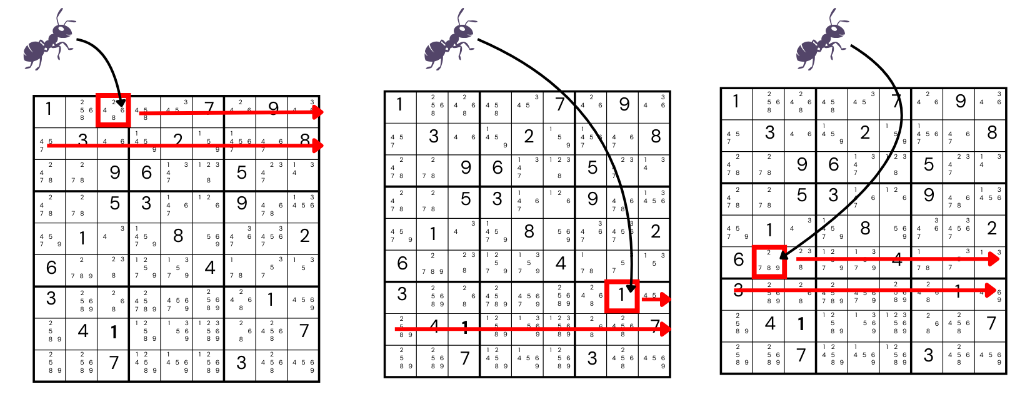
\includegraphics[width=0.9\textwidth]{../figures/Ants start.png}
            \centering
            \caption{Ants start at random cell}\label{Ants start}
        \end{figure}

    When the initial pass to the CP is done, the ants start their tour. The ants visit cell $i$ and check if the cell has already a fixed value assigned to it. If there is none, the ants look at the ``value set'' $v_i$, which contains all the valid candidate values for that cell. To choose a value $s$ from this set, ant depends on a random variable $q$ and compare this to $q_0$ which is a tunable parameter and whose value must be between $[0, 1]$. This random variable determines how greedy the ants should be. The value selection s is defined as follows:

        \begin{equation}
        s = \begin{cases} 
        \arg\max_{k \in v_i} \{ \tau_{i}^{k} \} & \text{if } q < q_0 \quad \text{(Greedy Selection)} \\
        S_{\text{roulette}} & \text{otherwise} \quad \text{(Roulette Wheel Selection)}
        \end{cases}
        \end{equation}

where $\tau_{i}^{k}$ is the pheromone value for assigning the value $k$ to cell $i$.

  \subsubsection*{Greedy and Roulette Wheel Selection}
\begin{center}
    \begin{minipage}{\linewidth}
        \centering
        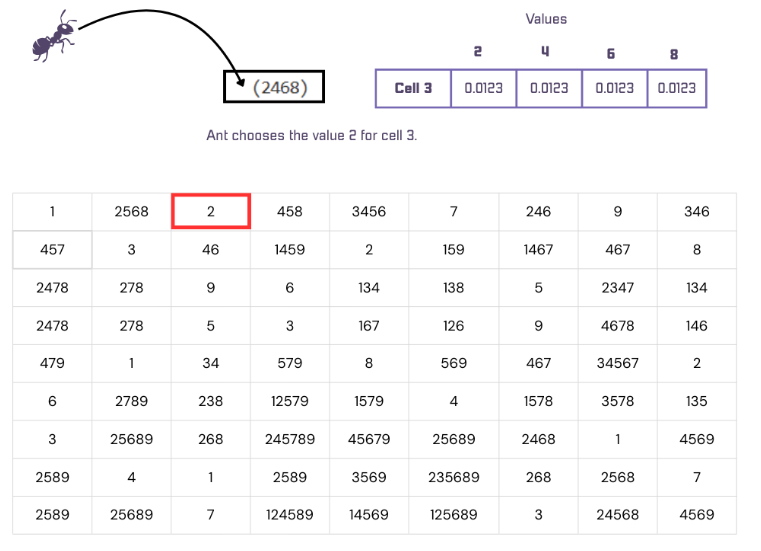
\includegraphics[width=0.8\linewidth]{../figures/Greedy Selection.png} 
        \captionof{figure}{Ants performs greedy selection} 
        \label{Ant Greedy} 
        
        \vspace{1.0cm} % Slightly smaller gap
        
        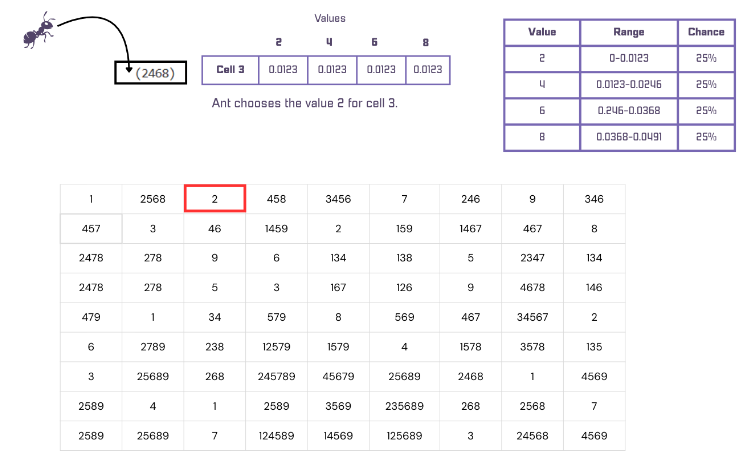
\includegraphics[width=0.8\linewidth]{../figures/Probabilities.png} 
        \captionof{figure}{Ants performs roulette wheel selection when $q \ge q_0$} 
        \label{Ant Roulette} 
    \end{minipage}
\end{center}

When $q \ge q_0$, the ants perform the roulette wheel selection instead of greedy selection (See Figure~\ref{Ant Greedy}). As opposed to the greedy selection, ants do not assign immediately the value that has the highest pheromone value for a certain cell. Instead, it calculates the probability $p_{i}^{k}$ of choosing the value $k$ and assigning it to the cell $i$ as shown in Figure~\ref{Ant Roulette}. The probability of each value getting picked from the value set depends on their pheromone values. However unlike the greedy selection, the value $s$ with low pheromone value still have a chance to be assigned to cell $i$.  The probability distribution is given by:

        \begin{equation}
        p_{i}^{k} = \frac{\tau_{i}^{k}}{\sum_{j \in v_i} \tau_{i}^{j}}
        \end{equation}

        where $k$ is a candidate value from the value set $v_i$. 

After the ant fixes the value for cell $i$, it calls the CP to propagate changes as shown in Figure~\ref{fig:cpacs_step_1b} and~\ref{fig:cpacs_step_2b}. Because of this, every after ant's step the CP further reduces the search space. It ensures that every next step, only valid candidates are chosen. This propagation also is significant in identifying that a certain move of the ant will lead to conflict (neighboring cells will have no valid candidate values anymore). That cell is considered fail cells.

\subsubsection*{Local Pheromone Update}

After the ants choose a value $s$ from the value set $v_i$ and assign it to cell $i$, they perform a \textbf{local pheromone update}. Then, the CP is called again to propagate the changes. The local pheromone update reduces the pheromone value of that assignment. It is done to purposely ``penalize'' that specific assignment as shown in Figure~\ref{Local Update}. Because of this, other ants have a low chance of choosing the same value for the same cell thus making the ants explore the other candidate values. 

The local pheromone update given by the following equation:

        \begin{equation}
        \tau_{i}^{s} \leftarrow (1-\xi)\tau_{i}^{s} + \xi\tau_{0}
        \end{equation}

where $\xi$ is the local pheromone evaporation coefficient, and $\tau_{0}$ is the initial pheromone value.

% --- CP Rule 1 ---
\begin{center}
    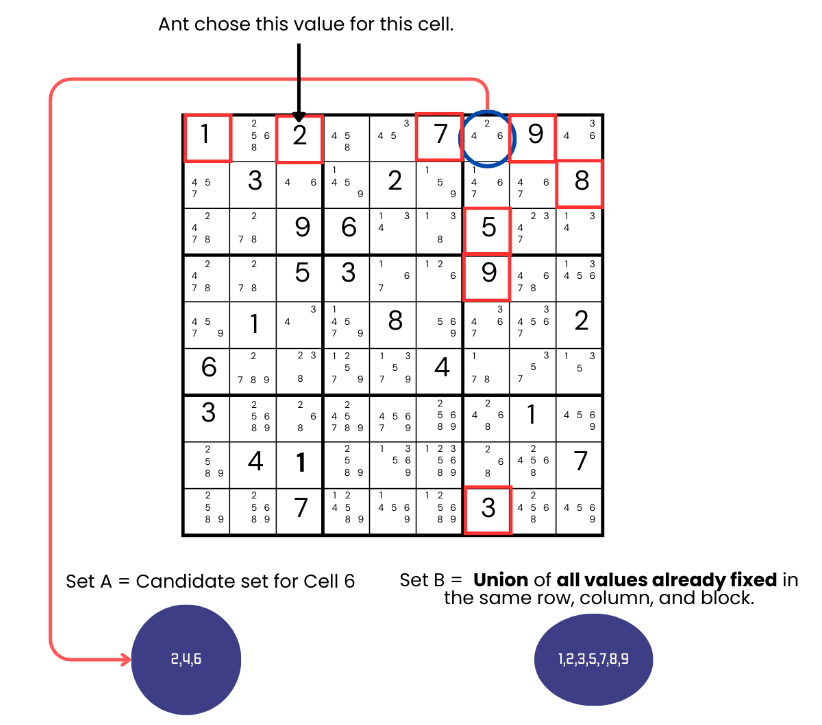
\includegraphics[width=0.65\linewidth]{../figures/CP in ACS Rule 1 a.png} 
    \captionof{figure}{Before applying CP Rule 1} 
    \label{fig:cpacs_step_1a} 
    
    \vspace{0.5cm} % Gap between images
    
    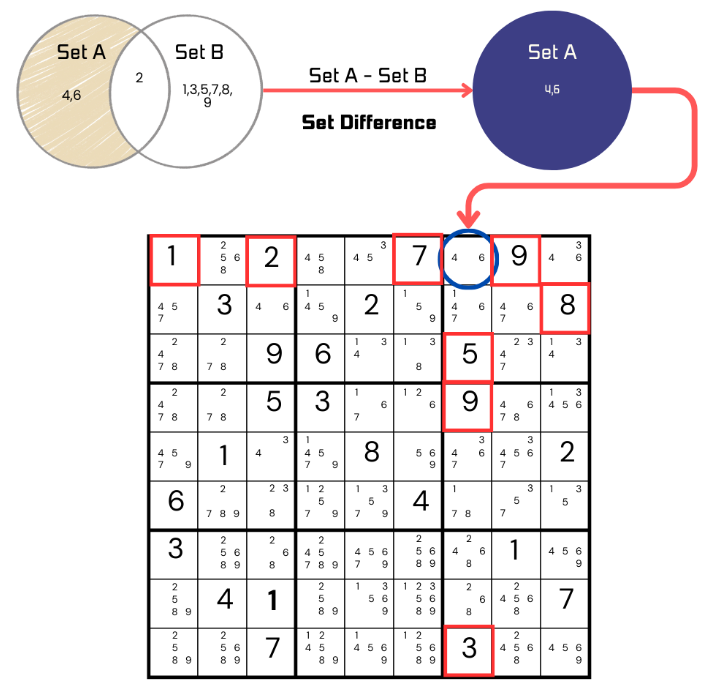
\includegraphics[width=0.65\linewidth]{../figures/CP in ACS Rule 1 b.png} 
    \captionof{figure}{After applying CP Rule 1} 
    \label{fig:cpacs_step_1b} 
\end{center}

\vspace{1cm} % Gap between Rule 1 and Rule 2

% --- CP Rule 2 ---
\begin{center}
    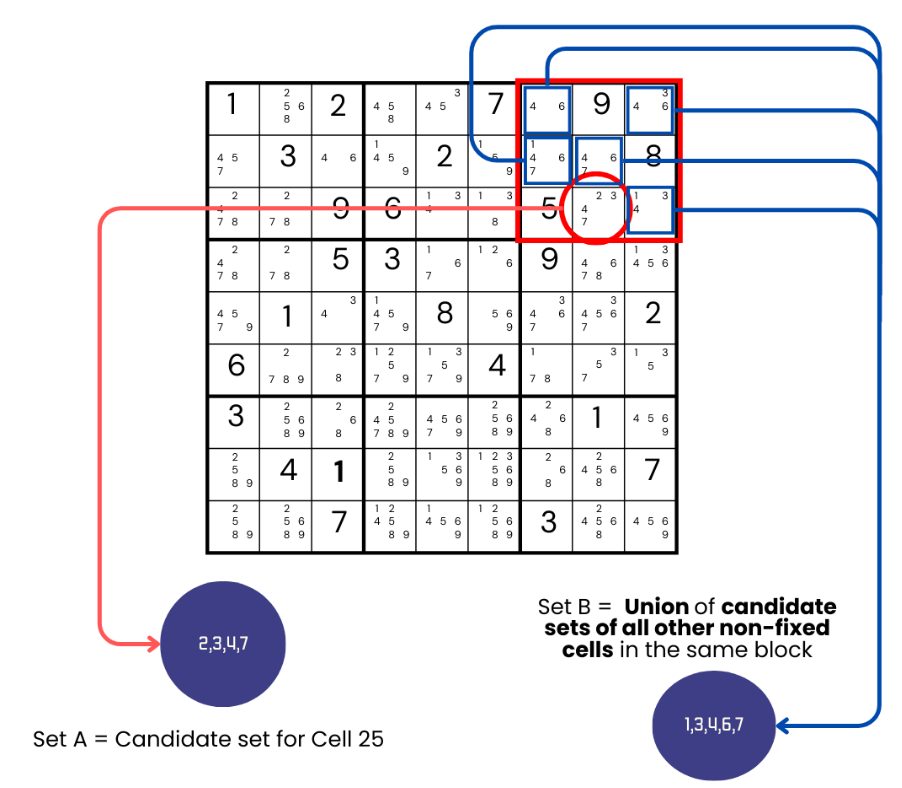
\includegraphics[width=0.65\linewidth]{../figures/CP in ACS Rule 2 a.png} 
    \captionof{figure}{Before applying CP Rule 2} 
    \label{fig:cpacs_step_2a} 
    
    \vspace{0.5cm} % Gap between images
    
    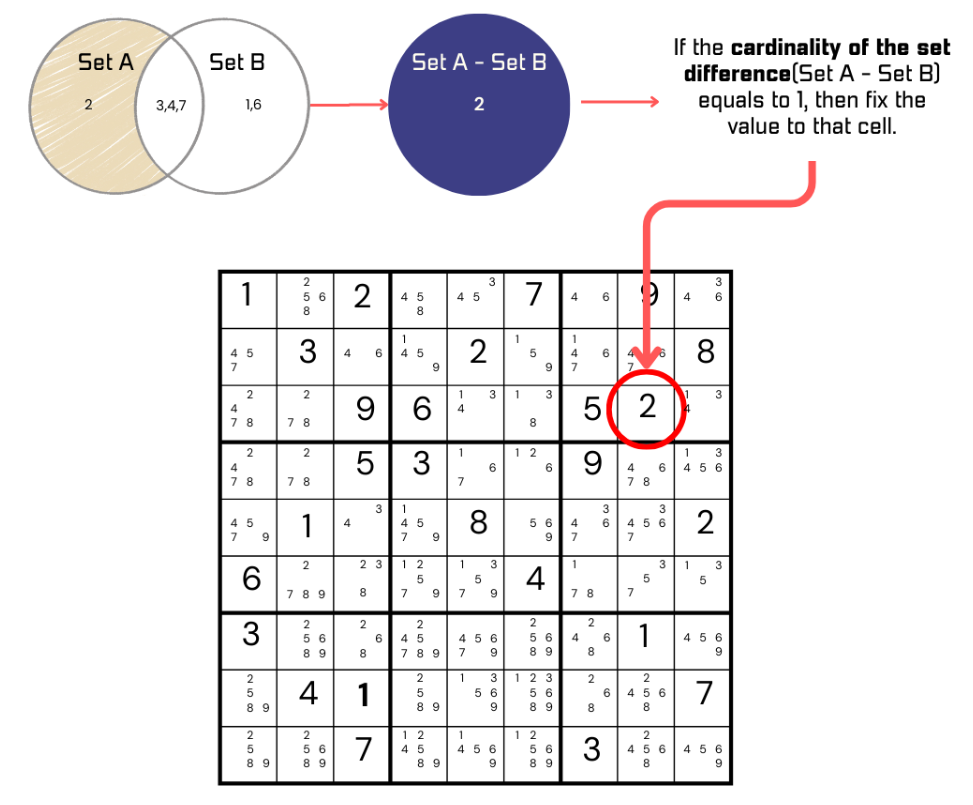
\includegraphics[width=0.65\linewidth]{../figures/CP in ACS Rule 2 b.png} 
    \captionof{figure}{After applying CP Rule 2} 
    \label{fig:cpacs_step_2b} 
\end{center}

        \begin{figure}[H]
            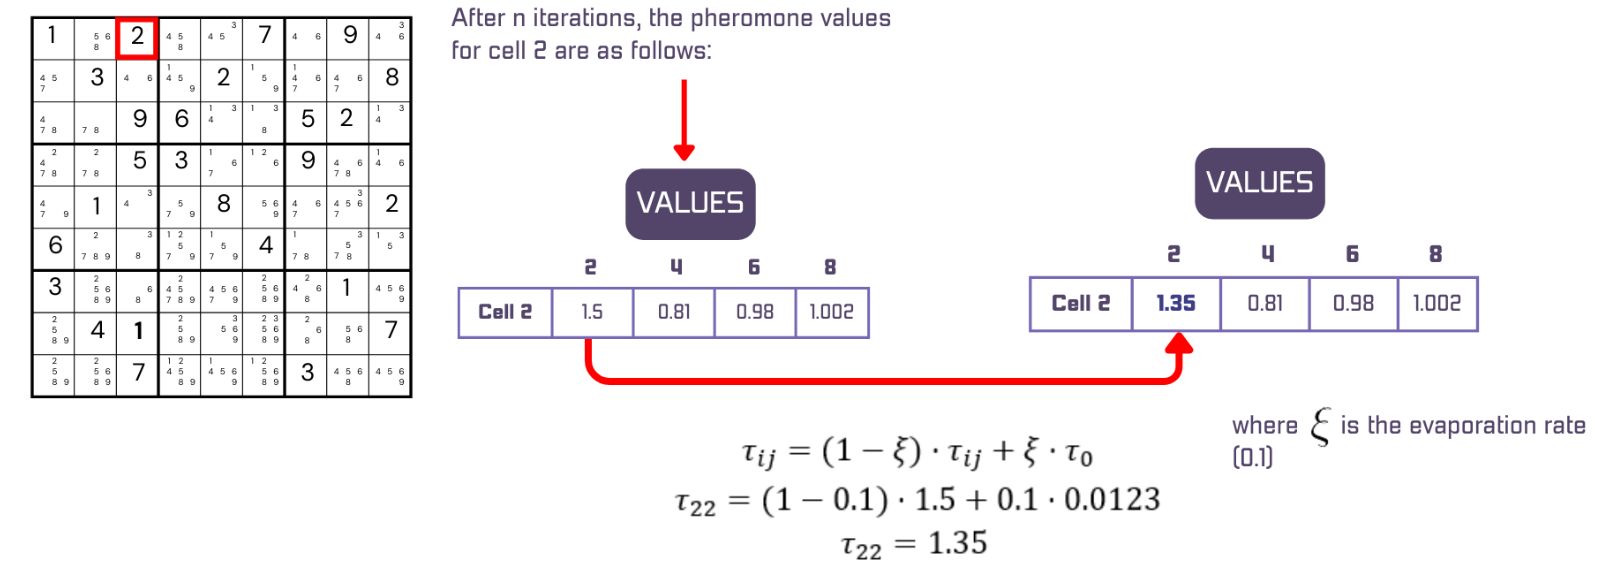
\includegraphics[width=0.9\textwidth]{../figures/Local Update.png}
            \centering
            \caption{Ant chooses the value $2$ for cell $2$}\label{Local Update}
        \end{figure}

\subsubsection*{Objective Function}
In TSP, the objective of any algorithm is often to minimize the cost of the tour. However, in the context of Sudoku, some ants may fail to solve a sudoku puzzle if they assigned a value to a certain cell that leads the subsequent cells to have no valid candidate value anymore. Therefore, sudoku should be complete in order to be considered as solved and this should also define the objective. 

        \begin{figure}[H]
            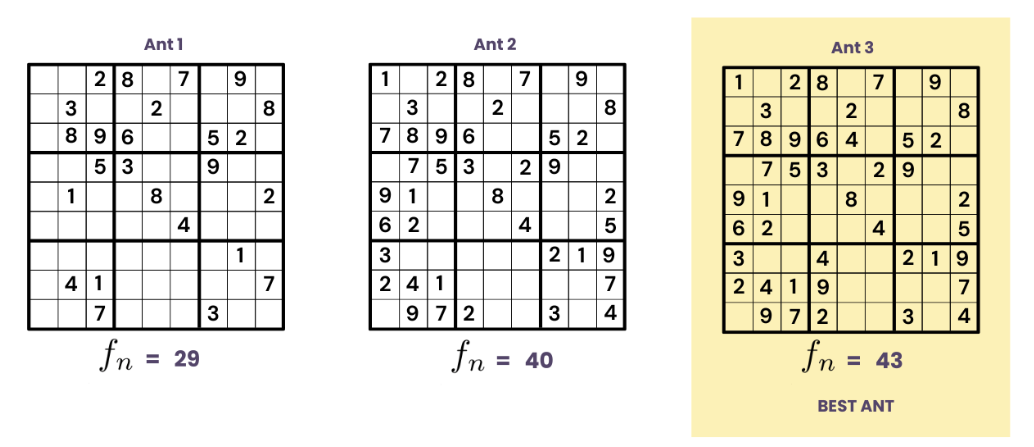
\includegraphics[width=\textwidth]{../figures/Finding Best Ant.png}
            \centering
            \caption{Finding the Best Ant}\label{finding best ant}
        \end{figure}

The number of cells filled by the ant $n$ is denoted by $f_n$. The objective of this proposed model focuses on maximizing the number of cells filled. The ant who has the highest number of filled cells is the iteration-best solution and is denoted by $f_{\text{best}}$ (See Figure~\ref{finding best ant}). Thus, the \textbf{objective function} of this research is given by:

        \begin{equation}
        f_{\text{best}} = \max_{n \in \{1 \dots m\}} f_n
        \end{equation}

        where $m$ is the total number of ants. The puzzle is solved only when $f_{\text{best}}$ becomes equal to the total number of cells in the puzzle.

\subsubsection*{Global Pheromone Update}

After the best ant is found, the solver does the \textbf{global pheromone update}. This is opposite from how the local pheromone update works because this global update is focused on exploitation rather than exploration. The most successful paths are given additional pheromone value computed from the global best solution. The solver does this update only after all the ants finish constructing a solution for the current iteration. 

The quality of the solution is determined by how close the solution is to completion. Adapted from the work of Lloyd and Amos~\cite{lloyd2020}, the pheromone deposit is calculated by the following equation:

        \begin{equation}
        \Delta \tau = \frac{N}{N - f_{best}}
        \end{equation}

where $N$ is the total number of cells in the puzzle and $f_{best}$ is the number of filled cells in the iteration-best solution. For example as shown in Figure~\ref{finding best ant}, the best ant was able to fill 43 cells out of 81 cell ($9 \times 9$ sudoku puzzle). Therefore, \textbf{$\Delta \tau = 2.131$}. 

This pheromone deposit, $\Delta \tau$, is then compared to the best pheromone deposit denoted as $\Delta \tau_{best}$ (initialized to 0). If $\Delta \tau$ is greater than the $\Delta \tau_{best}$, the solver replaces the value of the $\Delta \tau_{best}$ with the value of $\Delta \tau$ ($\Delta \tau_{best} = 2.131$). Similarly, the global-best solution is replaced with the iteration-best solution. The global pheromone update is then applied to the cell-value assignments (in our example the value 2 for cell 3) found in the global-best solution (See Figure~\ref{Global Update}). 

        \begin{equation}
        \tau_{i}^{s} \leftarrow (1-\rho)\tau_{i}^{s} + \rho \Delta \tau_{best}
        \end{equation}

where $\rho$ is the standard evaporation rate and whose value is between [0, 1].

This pheromone deposit $\Delta \tau_{best}$ is inversely proportional to the quality of the solution found. When the solution is nearly solved, the denominator decreases thus increasing the $\Delta \tau$. This makes the ants for the next iteration to be strongly influenced towards the paths that give an almost completed sudoku puzzle. 

        \begin{figure}[H]
            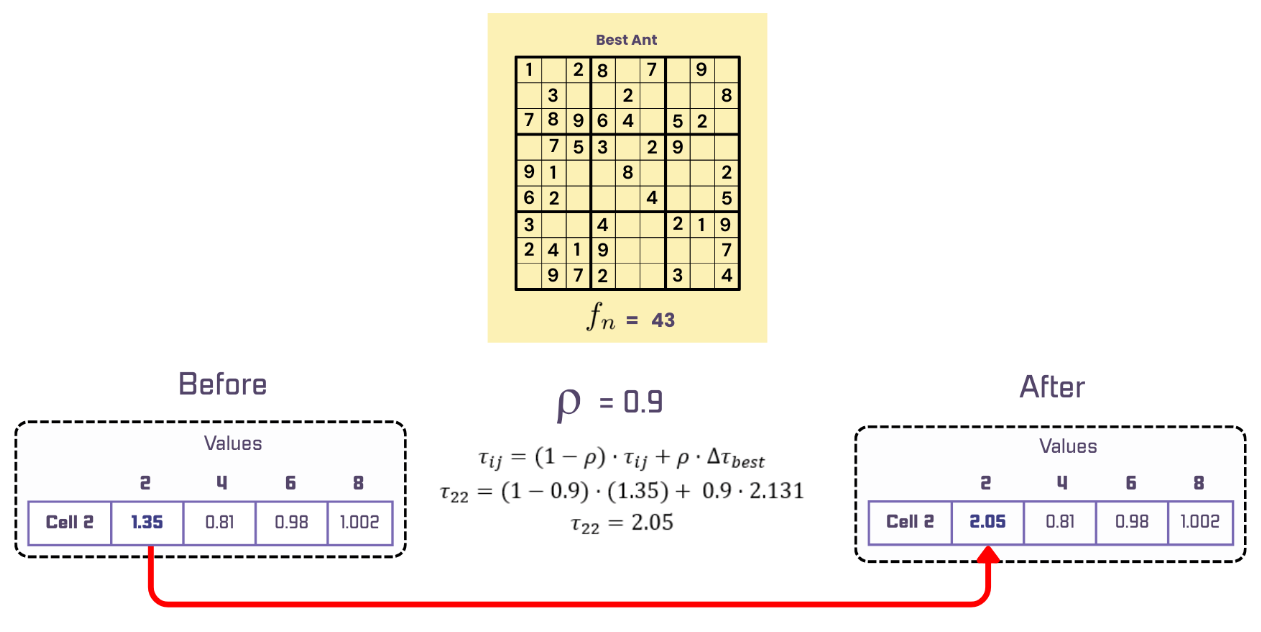
\includegraphics[width=0.9\textwidth]{../figures/Global Update.png}
            \centering
            \caption{Ant increases the pheromone value of the value $2$ for cell $2$}\label{Global Update}
        \end{figure}

        
       
\subsubsection*{Best Value Evaporation}
However, this global pheromone update can make the paths from the global-best solution so strong to the point that all the ants choose the same path. Because of this, exploration rapidly decreases and results in stagnation. Lloyd and Amos~\cite{lloyd2020} introduced the \textbf{best value evaporation (BVE)}. This is different from the standard evaporation rate from the global pheromone update as the BVE, shown in Figure~\ref{BVE}, is applied to decrease the value of the pheromone deposit $\Delta \tau_{best}$. It helps the ants ``forgets'' how good the global best solution was thereby encouraging the ants to explore other cell-value assignments. This is done every after the global pheromone update. 

        \begin{equation}
        \Delta \tau_{best} \leftarrow \Delta \tau_{best} \times (1 - \rho_{BVE})
        \end{equation}

        where $\rho_{BVE} \in [0,1]$ is a parameter controlling the decay rate.

        \begin{figure}[H]
            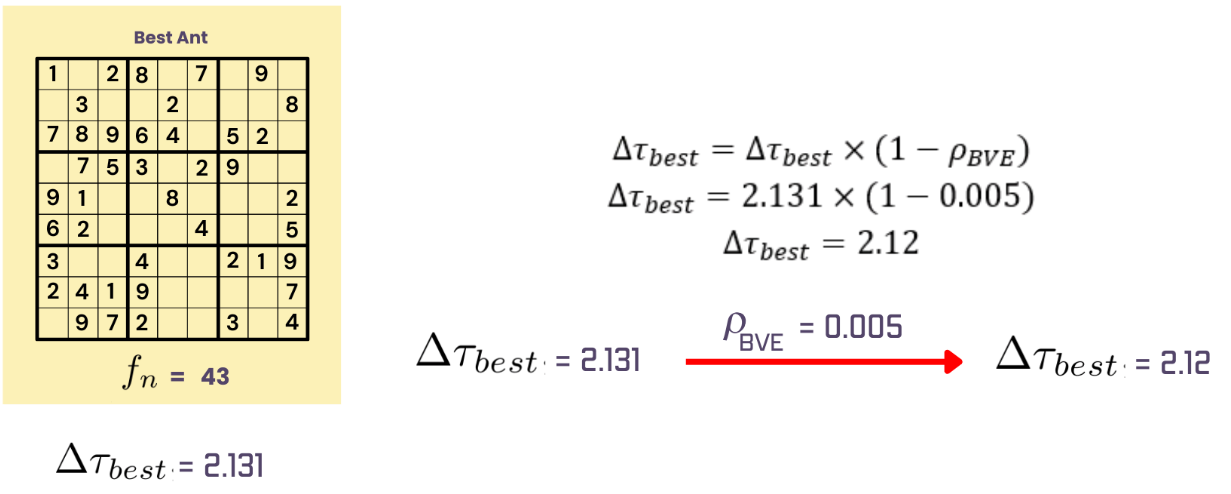
\includegraphics[width=0.9\textwidth]{../figures/BVE.png}
            \centering
            \caption{BVE decreases the value of $\Delta \tau_{best}$}\label{BVE}
        \end{figure}

\subsubsection*{Min-Max Ant System (MMAS)}
As the work of the ACS colony focuses on exploiting the best-so-far solution found, the Min-Max Ant System (MMAS) focuses on exploring the search space. This is a variant of ACO that has a unique search process (See Figure~\ref{MMAS Difference}). The first difference of this colony is the decision making. The ACS, as discussed above, chooses a value for a cell in two ways, either greedy selection or roulette wheel selection. MMAS colony chooses a value for a cell by roulette wheel selection only thus maintaining its exploratory characteristics. Because of this, the $q_0$ for this colony is always 0. 

        \begin{figure}[H]
            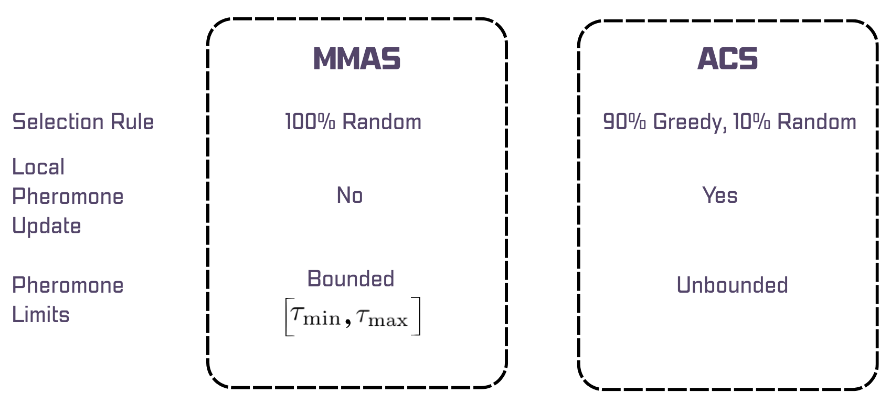
\includegraphics[width=0.9\textwidth]{../figures/MMAS Difference.png}
            \centering
            \caption{Difference Between MMAS and ACS}\label{MMAS Difference}
        \end{figure}
        
After it chooses a value, it doesn't have local pheromone update mechanism but it does the global pheromone update like the ACS colony. Furthermore, MMAS has no Best Value Evaporation and instead, it clamps the pheromone values to a certain range. For every cell-value $(i, j)$ assignment, there is a pheromone value associated with this which is denoted as $\Delta \tau_{i,j}$. This pheromone value should be within the range of $[\tau_{\min}, \tau_{\max}]$ as showin in Figure~\ref{MMAS Limits}~\cite{mo2022}.

The upper bound $\tau_{\max}$ and the lower bound $\tau_{\min}$ are computed as follows:
        \begin{equation}
        \tau_{\max} = \frac{1}{\rho} \cdot \left( {\Delta \tau} \right)
        \end{equation}

        \begin{equation}
        \tau_{\min} = \frac{\tau_{\max}}{2 \cdot N}
        \end{equation}

where $\rho$ is the evaporation rate and $N$ is the puzzle size (for example in $9 \times 9$ Sudoku puzzle, $N$ = 9).

        \begin{figure}[H]
            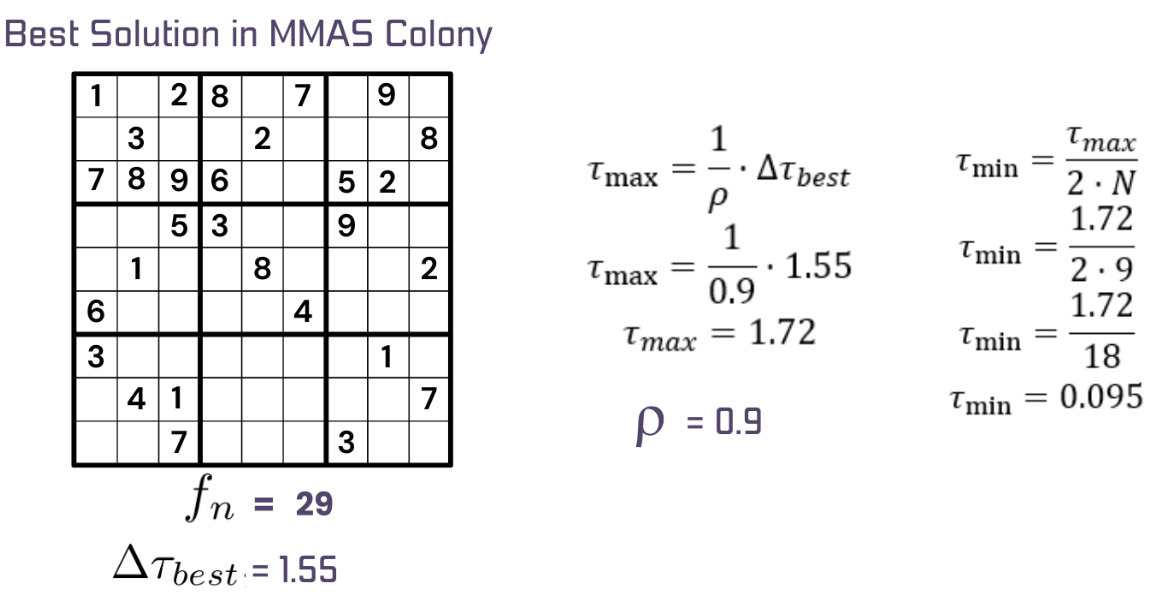
\includegraphics[width=0.9\textwidth]{../figures/MMAS Limits.png}
            \centering
            \caption{$\Delta \tau_{\max}$ and $\Delta \tau_{\min}$}\label{MMAS Limits}
        \end{figure}

If the $\Delta \tau_{i,j}$ becomes larger that the $\tau_{\max}$, then $\Delta \tau_{i,j}$ is set to $\tau_{\max}$. Similarly, if $\Delta \tau_{i,j}$ becomes smaller that the $\tau_{\min}$, then $\Delta \tau_{i,j}$ is set to $\tau_{\min}$. This limitations does not allow a cell-value assignment to accumulate large pheromone value thereby allowing more exploration. 

\subsubsection*{Dynamic Collaborative Mechanism}
As single-colony ant faces early convergence when it comes to more complex constraints, this paper adapts the heterogeneous multi-colony framework of~\cite{mo2022}. Figure~\ref{DCM-ACO Model} shows this framework which introduces multiple colonies running in parallel within a single thread. There will be one colony of Max-Min Ant System (MMAS) and $k$ colonies of Ant Colony System (ACS). This multi-colony framework balances the exploitation in which the ACS is responsible for and the exploration in which MMAS is better with. 

        \begin{figure}[H]
            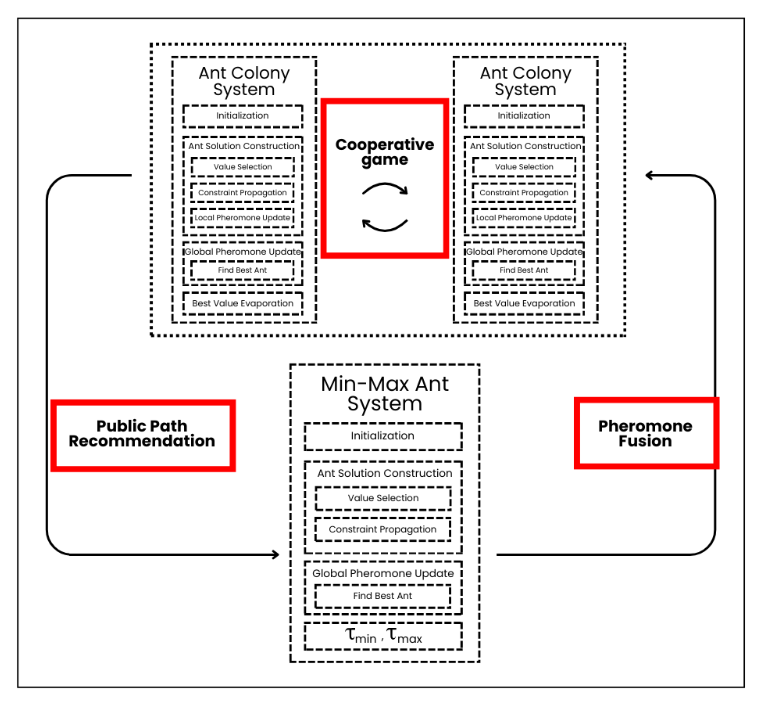
\includegraphics[width=0.9\textwidth]{../figures/DCM-ACO.png}
            \centering
            \caption{CP-DCM-ACO Model}\label{DCM-ACO Model}
        \end{figure}


        \subsubsection*{Cooperative Game Strategy }

        This strategy employs redistribution of pheromone based on the performance of the colonies and only applied to the ACS colonies. There is a ``payoff'' computed in this technique and it is the total pheromone deposits from the colonies. This payoff or total pheromone income is then fairly redistributed among the colonies based on their contribution~\cite{mo2022}. 
        
        The redistribution calculation proceeds in four steps:

        First, the pheromone deposit $\Delta \tau_{best}$ from all the ACS colonies are being added to calculate the total pheromone income denoted as $b$. 

        \begin{equation}
        b = \sum_{i=1}^{k} \Delta \tau_{ACS}^{i}
        \end{equation}

        Then, the entropy of each ACS colony is then calculated to determine their diversity using:
            \begin{equation} 
            P_i = \frac{k_i}{K} 
            \label{eqn:coop_game_2}
            \end{equation}
            \begin{equation} 
            E(t) = - \sum_{i=1}^{U} P_i \log P_i
            \label{eqn:coop_game_3}
            \end{equation}
        where $K$ represents number of ants in the ACS colony, $U$ is the number of unique solutions generated by ants, and $k_i$ represents the number of ants that generated the $i-$th unique solution. To simply put, a higher entropy value shows that the colony is in the state of exploration while lower entropy value indicates that the colony is in a state of exploitation thereby converging to a specific cell-value assignment. 
              
        The contribution of the $i$-th colony is determined by its solution quality ($sol_i$) and diversity ($H(p_i)$) as shown in Figure~\ref{Coop Game}. From the work of Mo et al.~\cite{mo2022}, the DCM-ACO was used to solve TSP.\@ So, to adapt the concept of ``tour length' to Sudoku, this study defines the length of a solution as the number of empty cells remaining ($numCells - f_i$, where $f_i$ is the number of filled cells and $numCells$ is the number of cells in the puzzle (81 for $9 \times 9$ puzzle)). The ratio between the global minimum length ($numCells - f_{best}$) to the colony's best length ($numCells - f_{i}$) defines the solution quality of the global-best solution from colony $i$. From this equation, colonies that is close to solving the puzzle receives higher quality score.

            \begin{equation}
            sol_i = \frac{numCells - f_{best}}{numCells - f_{i}}
            \end{equation}
            
        
            \begin{equation}
            H(p_i) = \frac{E(p_i)}{E(p_{\max})}
            \end{equation}

            where $E(p_{i})$ colony's entropy and $E(p_{\max})$ is the maximum entropy found among the ACS colonies.
        
        \begin{figure}[H]
            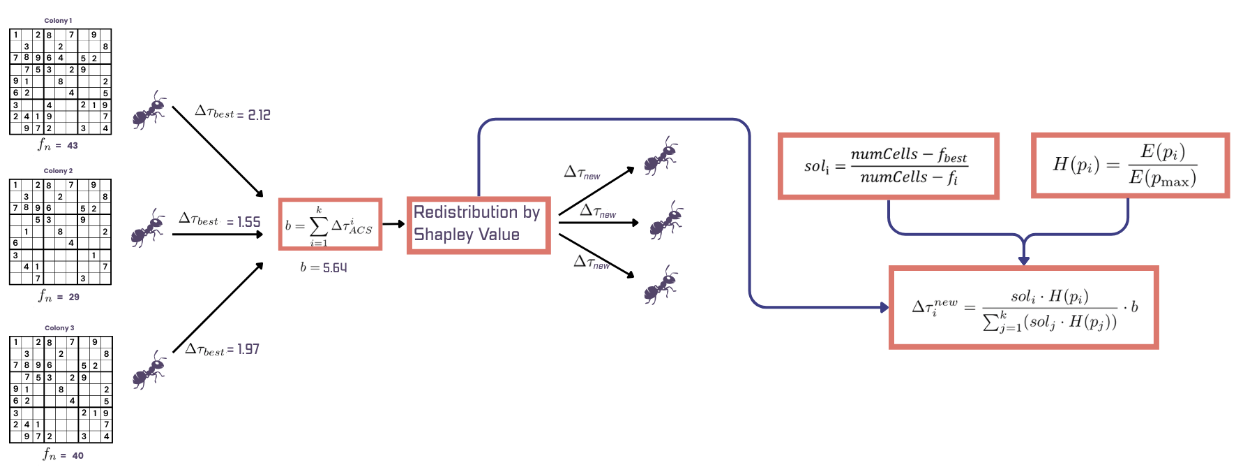
\includegraphics[width=0.9\textwidth]{../figures/Coop Game.png}
            \centering
            \caption{Cooperative Game Strategy}\label{Coop Game}
        \end{figure}

        Finally, the new pheromone deposit, $\Delta \tau_{i}^{new}$, is calculated for each ACS colony. This redistribution ensures that the colony that is performing well who has high diversity and good solution quality is rewarded and the poor-performing colony is punished (See Figure~\ref{Result}). 

        \begin{equation}
        \Delta \tau_{i}^{new} = \frac{sol_i \cdot H(p_i)}{\sum_{j=1}^{k} (sol_j \cdot H(p_j))} \cdot b
        \end{equation}

        \begin{figure}[H]
            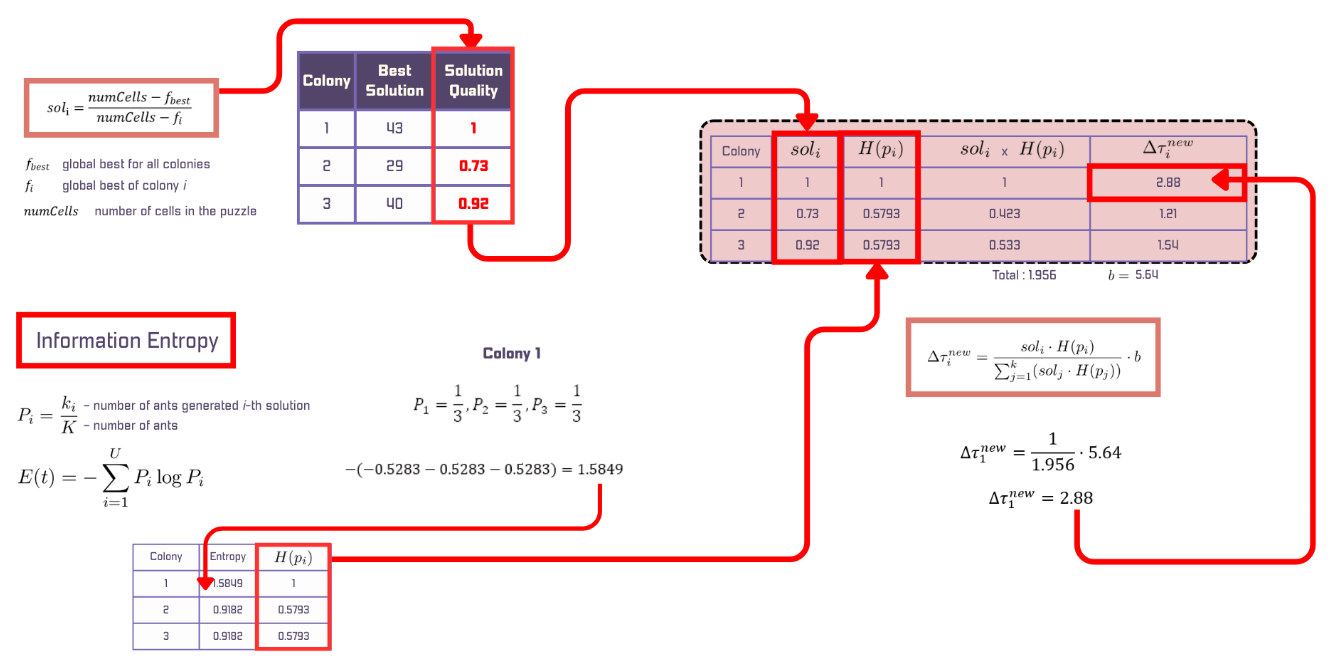
\includegraphics[width=1.0\textwidth]{../figures/Coop Game Result.png}
            \centering
            \caption{The Redistribution of Pheromone}\label{Result}
        \end{figure}


        \subsubsection*{Pheromone Fusion Mechanism}

        As mentioned earlier, ACS colonies are responsible for exploitation to maximize the number of filled cells. However, this process may lead the colony to stagnation. To resolve this, Mo et al.~\cite{mo2022} introduces the Pheromone Fusion Mechanism. This mechanism only triggers when the entropy $E(p_i)$ of the $i$-th ACS colony goes below the predefined threshold parameter, denoted as $E(p_i) < E^*(P)$. 
        
        Since information entropy indicates the diversity of the colony, going below the entropy threshold means the colony is in the state of stagnation. In this state, the ants are repeating the same cell-value assignments that lead to incomplete solutions. The algorithm must continuously monitor the entropy of each ACS colony to detect stagnation. When stagnation is detected, a weight factor $\omega_i$ is calculated to determine how strong the pheromone fusion is. 

        \begin{equation}
        \omega_{i} = \frac{E(P)_{ACS}^{i}}{E(P)_{ACS}^{i} + E(P)_{MMAS}}
        \end{equation}

        The fusion is done by updating the entire pheromone matrix of the ACS colony that was detected to be stagnant. Figure~\ref{Pher Fusion} shows that this update helps the stagnating ACS colony to explore other cell-value assignment as this update injects exploratory information from the MMAS colony to that ACS colony. 
        

        \begin{equation}
        ph_{ACS}^{i} \leftarrow (1-\omega_{i}) \cdot ph_{ACS}^{i} + \omega_{i} \cdot ph_{MMAS}
        \end{equation}

        where $ph_{ACS}^{i}$ represents the pheromone matrix of the $i$-th ACS colony and $ph_{MMAS}$ represents the pheromone matrix of the MMAS colony. 

        \begin{figure}[H]
            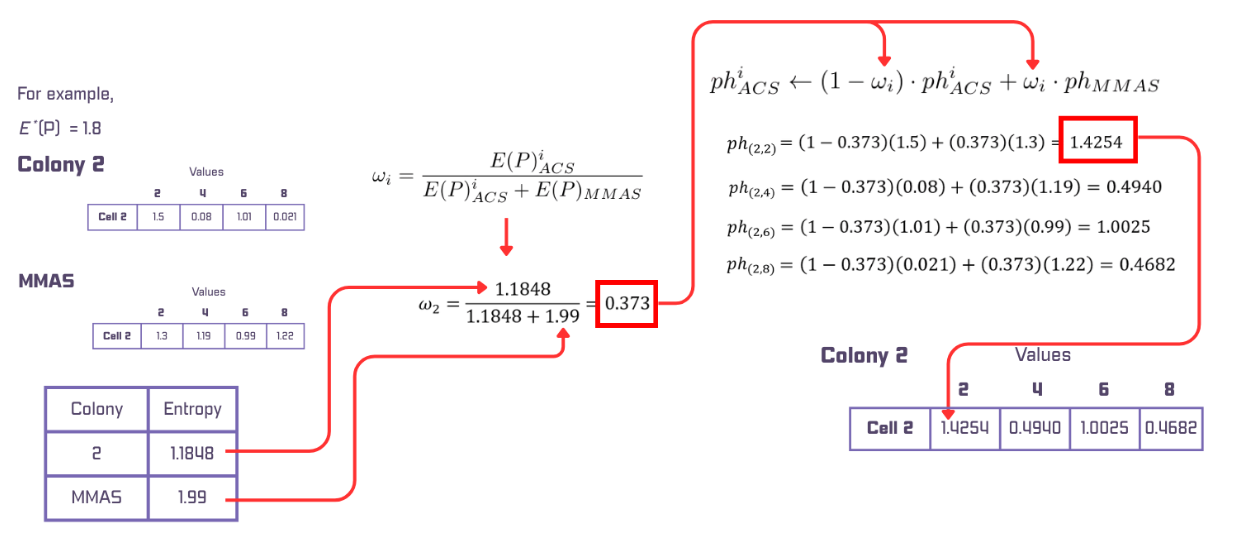
\includegraphics[width=0.9\textwidth]{../figures/Pher Fusion.png}
            \centering
            \caption{Pheromone Fusion}\label{Pher Fusion}
        \end{figure}

        \subsubsection*{Public Path Recommendation Strategy}

        While the MMAS colony is strong for exploration, it is not easy for this colony to converge as it will take longer time to lock onto a viable solution. This is the limitation that is being addressed by the public path recommendation strategy. In this strategy, ACS colonies ``recommend'' promising cell-value assignments to MMAS. However, in order to trigger this, a convergence rate ($con_t$) of the MMAS colony should be calculated and continuously be monitored~\cite{mo2022}. This rate is given by the ratio of the iteration number where the current optimal solution was found ($iter_{opt}$) to the current iteration number ($iter_t$).

        \begin{equation}
        con_t = \frac{iter_{opt}}{iter_t}
        \end{equation}

        This strategy is triggered when the algorithm detects that the convergence rate falls below the predefined convergence threshold denoted as ($con_t < con^*$). If this happens, it means the MMAS colony is struggling in solving the puzzle. A ``Public Path'' is then identified from the ACS colonies. This public path is a common cell-value assignment found from the best solution of the ACS colonies. For example, if all the ACS colonies have a cell-value assignment of (3, 4), then the algorithm will recommend this assignment to the MMAS colony by adding a pheromone value to this assignment in the MMAS pheromone matrix (See Figure~\ref{Public Path}). 

        The amount of this pheromone value to be added ($\tau_{public}$) is calculated based on the current iteration ($iter$). Because of this, the recommendation fades over time sustaining its natural exploratory characteristics. The formula, adapted from~\cite{mo2022}, for computing the pheromone value to be added is given by:

        \begin{equation}
        \tau_{public} = \frac{1}{N} \cdot e^{-iter}
        \end{equation}

        where $N$ is the puzzle size (for example in $9 \times 9$ Sudoku puzzle, $N$ = 9). 

        This calculated pheromone value is then added to the current pheromone value of recommended cell-value assignments ($i, j$)  in the MMAS pheromone matrix. This guides the MMAS colony to explore in this region of the solution space. 

        \begin{equation}
        \tau_{i,j}^{public} \leftarrow \tau_{i,j}^{public} + \tau_{public}
        \end{equation}

        where $\tau_{i,j}^{public}$ represents the pheromone value of the cell-value assignments ($i,j$) in the MMAS pheromone matrix. 

        \begin{figure}[H]
            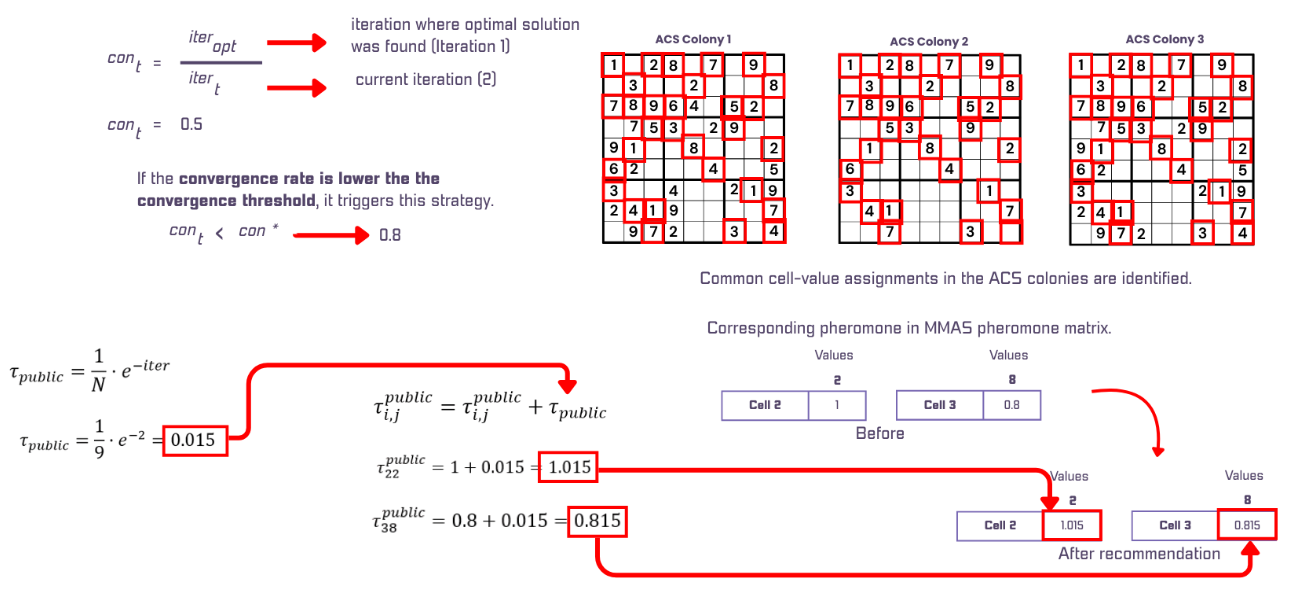
\includegraphics[width=0.9\textwidth]{../figures/Public Path.png}
            \centering
            \caption{Public Path Recommendation}\label{Public Path}
        \end{figure}

\subsection{Ring and Random Communication Topologies}
The proposed model of this study, multithreaded multi-colony ant optimization with ring and random communication topologies, builds up from the base model, CP-DCM-ACO. It introduces a parallel framework where there are multiple instances of the base model running separately in threads. These threads are going to terminate their process if one of them has already solved the puzzle by the common termination flag that is shared among all of them. 
        
The communication between the threads are adapted from how the processors communicate in the work of Yang and Fang~\cite{yang2015}. They introduced two ways of communication topologies namely ring topology and random-matching topology. In this framework, the master thread is not going to collect and organize the solutions from the slave threads. Instead, it has equal status with the slave threads in terms of searching the solution space. However, an additional task is given to the master thread and that is to create a random sequence of all the thread IDs and broadcast it to all the slave threads.


When the collaboration between threads are triggered, each thread prepares their iteration-best solution and global best solution. Since the base model used in this study is the multi-colony ant optimization and there are multiple colonies within each thread, the iteration-best solution of each colony is compared and the best one is the one that will be used for collaboration between threads. Similarly, the best among the best-so-far solutions from all the colonies within the single threads is used for this inter-thread communication. Each thread follows the following pattern for collaboration:
        
        \begin{enumerate}
            \item \textbf{Ring Topology} --- Thread $i$ sends its iteration-best solution to thread $(i + 1) \bmod n$, and receives an iteration-best solution from the previous thread $(i - 1 + n) \bmod n$.
            \item \textbf{Random-Matching Topology} ---  After each thread found its own ID in the broadcasted permutation of the thread IDs by the master thread, then it:
            \begin{itemize}
                \item sends its best-so-far solution to the thread whose ID is found in $\text{array}[(i + n + 1) \bmod n]$, and
                \item receives a best-so-far solution from the thread whose ID is found in $\text{array}[(i - n + 1) \bmod n]$.
            \end{itemize}
        \end{enumerate}


        \begin{figure}[H]
            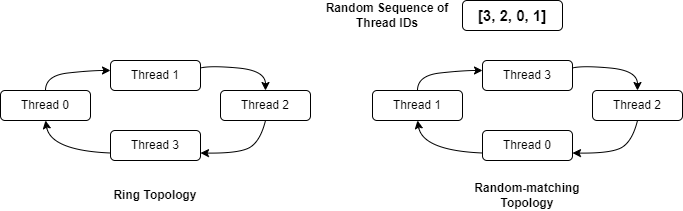
\includegraphics[width=\textwidth]{../figures/Topologies.png}
            \centering
            \caption{Ring Topology and Random-matching Topology}\label{Topology}
        \end{figure}

Figure~\ref{Topology} illustrates the ring and random-matching topologies used in the proposed model. Instead of exchanging the entire pheromone matrix between threads, only the path information or the cell-value assignments are being sent. Yang and Fang~\cite{yang2015} stated that by doing this, communication overhead between threads is reduced while maintaining cooperation. After each thread receives two best solutions from other threads, they use this information to update the pheromone matrix of the MMAS colony only. External pheromone reinforcement to the ACS colonies may disrupt the cooperative game strategy. This external pheromone update may alter the original diversity of the ACS colonies when the information entropy is quantified. The update on the pheromone matrix of the MMAS colony for each thread is given by:

        \begin{equation}
            \Delta \tau_{ij} = \Delta \tau^{(1)}_{ij} + \Delta \tau^{(2)}_{ij} + \Delta \tau^{(3)}_{ij}
        \end{equation}
        
        \begin{equation}
            \tau_{ij} = (1 - \rho)\tau_{ij} + \rho\Delta \tau_{ij}
        \end{equation}

where $\rho$ is the pheromone evaporation rate, and $\tau_{ij}$ is the pheromone value of the value $j$ to cell $i$. The total pheromone deposit $\Delta \tau_{ij}$ consists of three components:

        \begin{enumerate}
            \item $\Delta \tau^{(1)}_{ij}$ --- reinforcement from the thread’s own iteration-best solution;
            \item $\Delta \tau^{(2)}_{ij}$ --- reinforcement from the iteration-best solution received from its ring neighbor; and
            \item $\Delta \tau^{(3)}_{ij}$ --- reinforcement from the best-so-far solution received from a randomly-matched neighbor.
        \end{enumerate}

        \begin{figure}[H]
            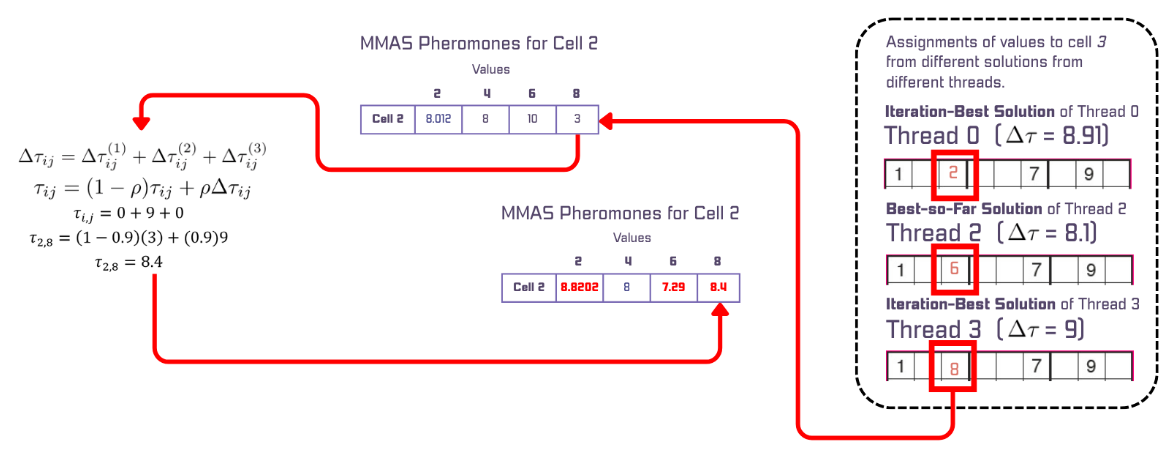
\includegraphics[width=0.9\textwidth]{../figures/Threads Result.png}
            \centering
            \caption{Thread 0 updates pheromone levels of the values from the candidate values on cell 2 based on the received solutions from Thread 2 and 3 using equation (23) and (24).}\label{Thread Comms}
        \end{figure}

This pheromone influence from other threads, as shown in Figure~\ref{Thread Comms}, allows the MMAS to accept external information about the other region of the solution space. Although the ACS colonies are not using this information, they are still indirectly influenced by this when the pheromone fusion mechanism is triggered. Because of this, the exploration to the solution space has greatly increased making this framework effective for solving complex sudoku puzzles.
    
\subsubsection*{Stopping Criteria}
The algorithm stops its execution once there is a thread that has already solved the sudoku puzzle. If any of the threads had constructed a complete and valid sudoku solution, it triggers the stopFlag to true, sending the signal to other concurrent threads to stop. A predefined time is also set in case threads are struggling to find a solution. If the execution time exceeds the predefined time, the algorithm is forced to terminate.


\section{Model Deployment Details}

The model is deployed as a web-based application using Flask and C++. The application allows the user to manually input numbers to the sudoku puzzle or remove numbers from a solved puzzle. There is also a list of instances a user can choose instead of creating their own puzzle. The application also allows the user to change the values of the parameter used by the solver in the back-end. Upon solving, the application allows the visualization of how the solver updates the values in the puzzle. This allows the user to observe how the solver converges to a final valid solution real-time (See Figure~\ref{deployment}).

        \begin{figure}[H]
            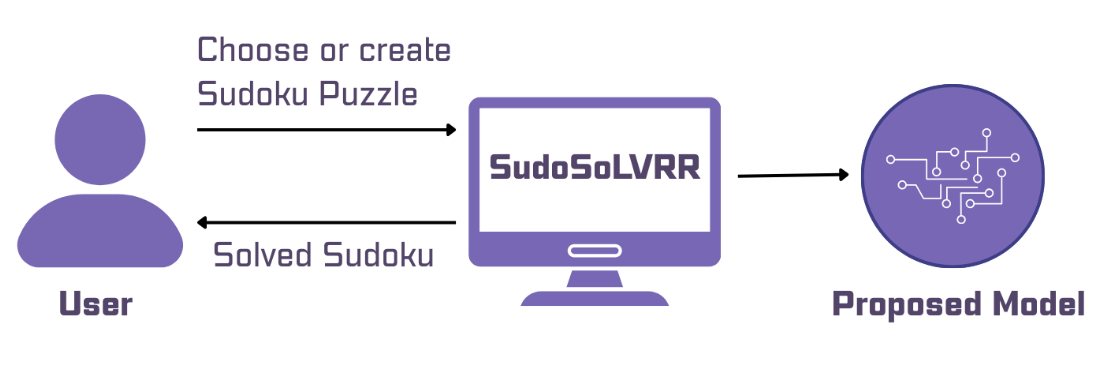
\includegraphics[width=0.9\textwidth]{../figures/SudoSoLVRR.png}
            \centering
            \caption{Model deployment as Web-based application}
            \label{deployment}
        \end{figure}